\section{Materiales y métodos}

    Se estudió la respuesta en frecuencia de un circuito en serie que permitía alternar entre configuraciones RC y RLC mediante un interruptor que puenteaba al inductor. El circuito RC visto desde la resistencia funciona como un filtro de frecuencias por encima de los \SI{1500}{\hertz}, en cambio, visto desde el capacitor filtra un rango de frecuencias de hasta \SI{1300}{\hertz}. En esta experiencia, se contó con una resistencia comercial de \SI{1}{\kilo\ohm}, un capacitor comercial de \SI{100}{\nano\farad} y un inductor $L$ de inductancia desconocida. 
    
Se utilizó como fuente una señal sinusoidal de amplitud constante mediante un generador de funciones $Sinometer$ modelo VC2002 \cite{VC2002}, variando su frecuencia en un rango de [0,1, 50] \SI{}{\kilo\hertz}. Tanto la señal de entrada (CH1) como la de salida (CH2) se registraron a través de un osciloscopio $Tektronix$ modelo TDS 220 \cite{TDS200}, que permitió medir las diferencias de potencial sobre ambos elementos simultáneamente, colocando el negativo de ambos sobre un punto común (ver \autoref{fig:circuito}). 
\begin{figure}[H]
\centering
\begin{minipage}{0.5\textwidth}
    \centering
    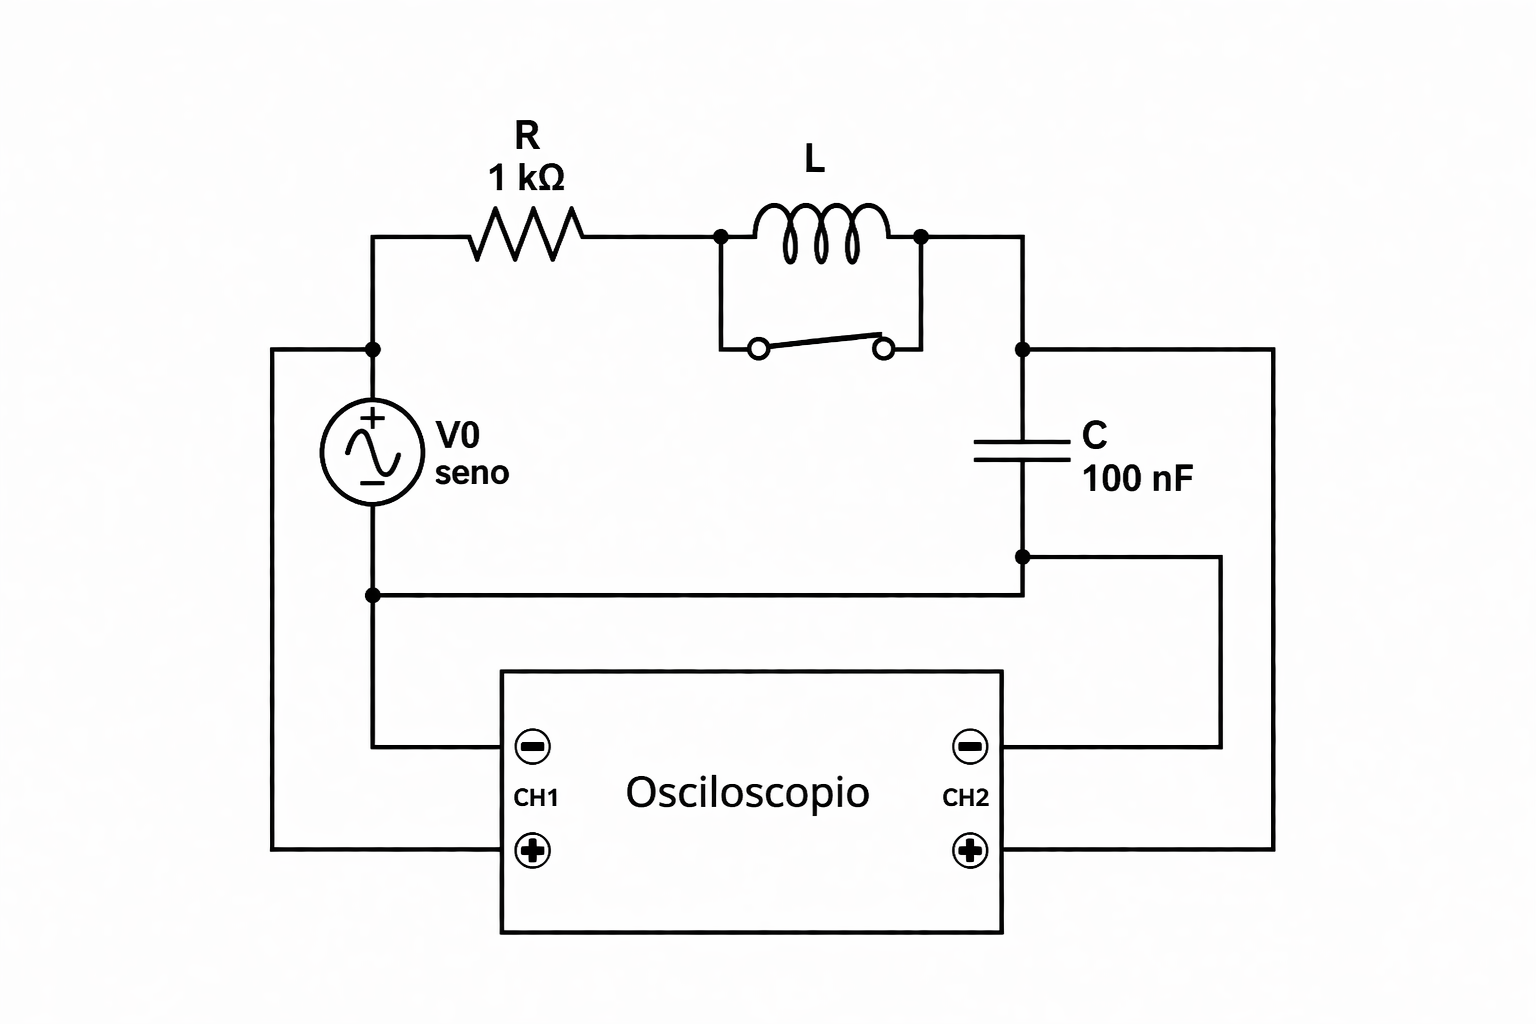
\includegraphics[width=\linewidth]{gráficos/Circuito.png}
    \caption{Esquema del circuito RLC en serie conectado al generador de señal y al osciloscopio. Se obtiene la configuración RC del circuito al cerrar el interruptor, mientras que si el interruptor está abierto se trata de la configuración RLC del mismo. En el canal uno (CH1) se conectó a la fuente, mientras que el canal dos (CH2) se conectó a la salida.}
    \label{fig:circuito}
\end{minipage}
\hfill
\begin{minipage}{0.45\textwidth}
    Para la configuración RC (interruptor cerrado), se realizaron medidas de la tensión de salida tanto sobre la resistencia como sobre el capacitor, permitiendo estudiar el filtro pasa-altos y el pasa-bajos, respectivamente. Para la configuración RLC (interruptor abierto), las mediciones se hicieron únicamente sobre la resistencia. 
    Para cada frecuencia se determinaron las amplitudes de las señales de entrada y salida. El desfasaje \(\varphi\) entre ambas señales se obtuvo a partir de la relación \(\varphi = 2\pi f \Delta t\), siendo $f$ la frecuencia de la fuente y $\Delta t$ la diferencia temporal entre ellas.  A partir de los datos obtenidos se calculó el módulo de la función de transferencia $H(\omega)$, como el cociente entre las amplitudes de entrada y salida, y la tangente del desfasaje $\varphi$. 
\end{minipage}
\end{figure}

Para el circuito RC, se estimó la frecuencia de corte, característica del circuito, a partir de $\omega_0=\frac{1}{\tau}$, siendo que $\tau = RC$, y se realizó un barrido de frecuencias que abarcó aproximadamente una década por debajo y una por encima de ese valor.  Experimentalmente, se buscó determinar  $\omega_0$, considerando que es aquella para la cual la función de transferencia cumple $|H(\omega_c)|= \frac{1}{\sqrt{2}}$. Esto corresponde a una disminución de la potencia a la mitad, dado que $P\propto |H|^2$. Utilizando el hecho de que en los regímenes de bajas y altas frecuencias la función $H(\omega)$ presenta comportamientos simples (aproximadamente constante en uno de los extremos y proporcional a una potencia de $\omega$ ($\omega$ para el pasa altos y $\omega^{-1}$ para el pasa bajos en el otro), que se traducen en rectas en escala logarítmica,  se representó el $\text{log}(H)$ en función del $\text{log}(\omega)$. Fueron realizados ajustes lineales en las dos regiones diferenciadas, estimando la frecuencia de corte a partir de la intersección de dichas rectas, pues es una buena aproximación al punto donde la función $|H(\omega)|$ alcanza el valor $\frac{1}{\sqrt{2}}$.  

En el caso del circuito RLC, se efectuó un barrido de frecuencias en el rango de [0, 50] \SI{}{\kilo\hertz}, donde se identificó la frecuencia de resonancia experimentalmente como aquella en la que el módulo de la función de transferencia $H(\omega)$ alcanza un máximo.  Para esta configuración del circuito, se construyó un gráfico de $|H(\omega)|$ en función de $\omega$ cuyo máximo corresponde a la frecuencia de corte. De esta manera, se determinó la inductancia del circuito según $\omega_r=\frac{1}{\sqrt{LC}}$. 

 %Para el circuito RC se buscó determinar la frecuencia de corte $\omega_c$, definida como aquella para la cual la función de transferencia cumple $|H(\omega_c)|= \frac{1}{\sqrt{2}}$, lo que corresponde a una disminución de la potencia a la mitad, dado que $P\propto |H|^2$. Utilizando el hecho de que en los regímenes de bajas y altas frecuencias la función $H(\omega)$ presenta comportamientos simples (aproximadamente constante en uno de los extremos y proporcional a una potencia de $\omega$ ($\omega$ para el pasa altos y $\omega^{-1}$ para el pasa bajos en el otro), que se traducen en rectas en escala logarítmica,  se representó el $\text{log}(H)$ en función del $\text{log}(\omega)$. Fueron realizados ajustes lineales en las dos regiones diferenciadas, estimando la frecuencia de corte a partir de la intersección de dichas rectas, pues es una buena aproximación al punto donde la función $|H(\omega)|$ alcanza el valor $\frac{1}{\sqrt{2}}$.  

 Finalmente, para ambas configuraciones se construyeron diagramas de Nyquist a partir de la gráfica de las componentes $H(\omega)$ en el plano complejo, siendo $Re(H)=H\cos(\varphi)$ y $Im(H)=H\sin(\varphi)$.